\documentclass[12pt, oneside]{article}
\usepackage{soto-quiz}
\usepackage{tikz}
\usepackage{fancyhdr}

\newif\ifsolution
\input{solution}

\begin{document}

\lhead{ENSP 202}
\chead{Exercises 5}
%\rhead{\today}
\rhead{Wednesday 26 Mar 2014}
\lfoot{}
\cfoot{}
\rfoot{}
\pagestyle{fancy}

\namebox

\problem{Exponential Growth}

The mass of mold on my pizza is 2 grams right now.  Mold scientists tell
me it will grow according to the function

$$ \textrm{Mold (grams)} = 2 e^{0.08 t} $$

Where $t$ is the number of hours from now.

How many grams of mold will
there be in a twelve hours?

\solution{

$$ 2 e^{0.08 \cdot 12} = 5.2 $$

5.2 grams or almost triple.

}

How long until I have 20 grams of mold?

\solution{
This requires a little bit of algebra.  The question we ask is, what is
$t$ when the amount of mold equals 20 grams?

$$ 20 grams = 2 e^{0.08 t} $$
$$ 10 = e^{0.08 t} $$

Recall what the natural log function tells us: If $y = e^x$ then $\ln y = x$

$$ ln 10 = 2.3 = 0.08 \cdot t $$
$$ t = 2.3/0.08 = 29 hours $$

}


\problem{Graphing slopes}

We measure the depth of a tub of dimensions 1 meter by 0.5 meters.
Sketch the flow rate of the faucet into the tub in the second graph.

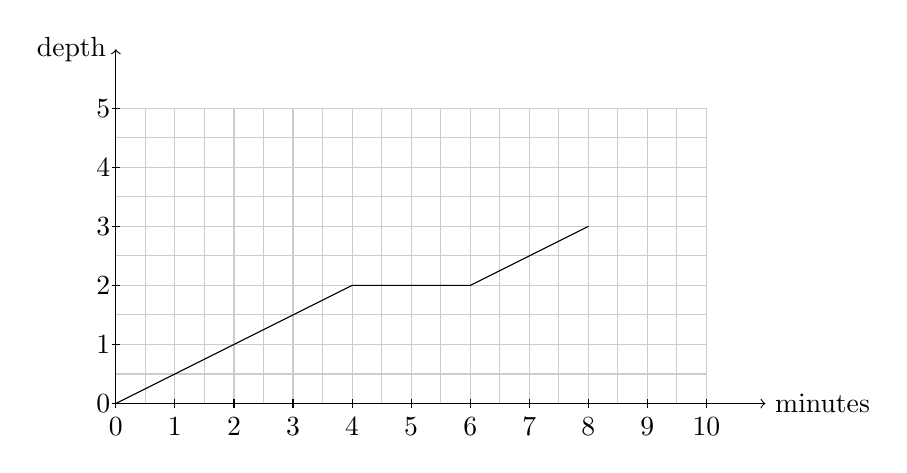
\begin{tikzpicture}[scale=0.75]
\def\sx{1}
\def\sy{1}

% tikz problem with grid to figure out slopes of graph
% Draw thin grid lines with color 40% gray + 60% white
\draw [step=0.5,thin,gray!40] (0, 0) grid (10, 5/\sy);

% Draw x and y axis lines
\draw [->] (0, 0) -- (11.0, 0) node [right] {minutes};
\draw [->] (0, 0) -- (0, 6/\sy) node [left] {depth};

% voltage labels
\foreach \x in {0,1,2,3,4,5,6,7,8,9,10} {
    \draw (\x/\sx, 2pt) -- (\x/\sx,-2pt) node[below] {$\x$};
}

\foreach \y in {0,1,2,3,4,5} {
    \draw (-2pt,\y/\sy) -- (2pt,\y/\sy) node[left] {$\y$};
}



\draw (0,0) -- (4,2) -- (6, 2) -- (8, 3);

\end{tikzpicture}


\solution{
We want to find the rate at which water is being poured into the tub in
volume per minute.  We need to convert our depth into the volume of
water.  To do this we use the estimation that the volume is the length
times the width of the tub times the depth of the water.

We use the depth to find the volume.  Over the first four minutes, the
depth increases from 0 to 2 meters.
The volume then is
$$ V = l \cdot w \cdot depth$$
$$ V = 1m \cdot 0.5m \cdot 2m = 1.0 m^3 $$

The rate is then

$$ \frac{1.0 m^3}{4 min}= 0.25 m^3/min $$

Over the period of time from 4 to 6 minutes, the depth does not increase
so the flow must be zero.  From 6 to 8 minutes the slope is the same.
In a graph, the flow looks like:

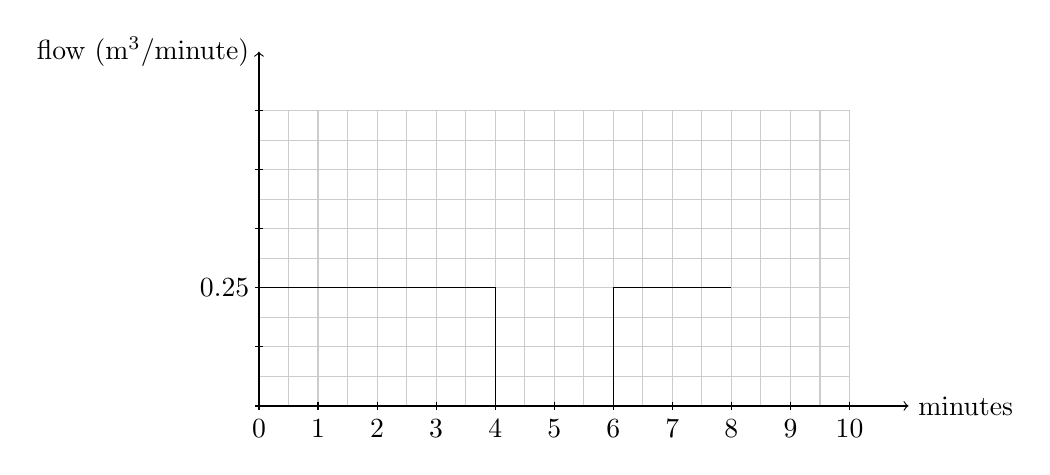
\begin{tikzpicture}[scale=0.75]
\def\sx{1}
\def\sy{1}

% tikz problem with grid to figure out slopes of graph
% Draw thin grid lines with color 40% gray + 60% white
\draw [step=0.5,thin,gray!40] (0, 0) grid (10, 5/\sy);

% Draw x and y axis lines
\draw [->] (0, 0) -- (11.0, 0) node [right] {minutes};
\draw [->] (0, 0) -- (0, 6/\sy) node [left] {flow (m$^3$/minute)};

% voltage labels
\foreach \x in {0,1,2,3,4,5,6,7,8,9,10} {
    \draw (\x/\sx, 2pt) -- (\x/\sx,-2pt) node[below] {$\x$};
}

\foreach \y in {0,1,2,3,4,5} {
    \draw (-2pt,\y/\sy) -- (2pt,\y/\sy) node[left] {};
}

\draw (0,2) node[left] {0.25};

\draw (0, 0) -- (0,2) -- (4,2) -- (4,0) -- (6,0) -- (6,2) -- (8,2) ;


\end{tikzpicture}

}


\end{document}

